\documentclass[showpacs,preprintnumbers,amsmath,amssymb,letter]{revtex4}

\usepackage{graphicx}% Include figure files
\usepackage{dcolumn}% Align table columns on decimal point
\usepackage{bm}% bold math
\usepackage{pst-all} 
\usepackage{SIunits} 
\usepackage{calc}

\normalsize
\setlength{\voffset}{\baselineskip*5}
\setlength{\textheight}{\baselineskip*53+\topskip}
\setlength{\hoffset}{0pt}
\setlength{\oddsidemargin}{40pt}
\setlength{\evensidemargin}{82pt}
\setlength{\textwidth}{380pt}

\newcommand{\vc}{\mathbf c}
\newcommand{\vrr}{\mathbf r}
\newcommand{\vu}{\mathbf u}

\begin{document}
\thispagestyle{empty}
\begin{figure}
%GNUPLOT: LaTeX picture with Postscript
\begin{picture}(0,0)%
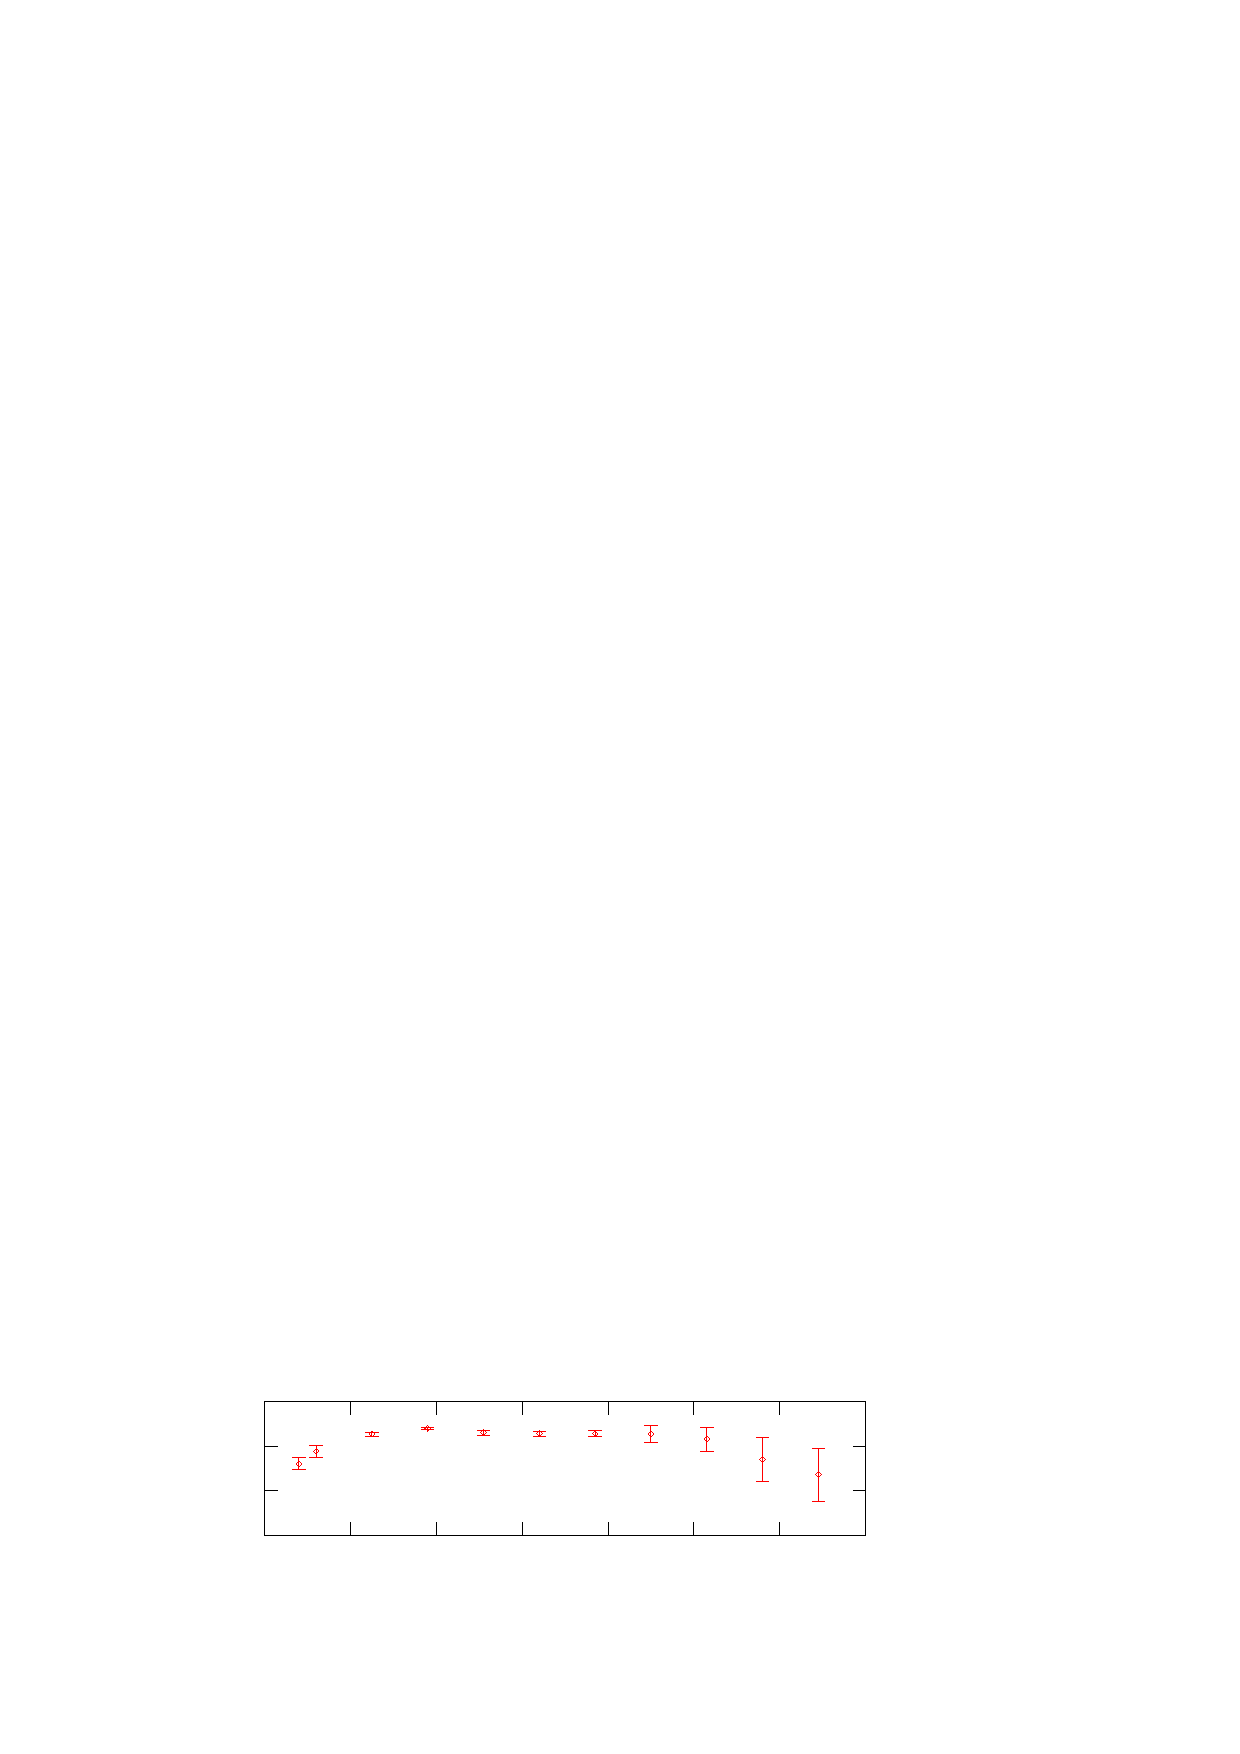
\includegraphics{Fo-equilibrium-amplitud-rounded-ys-yn}%
\end{picture}%
\begingroup
\setlength{\unitlength}{0.0200bp}%
\begin{picture}(18000,5400)(0,0)%
\put(2475,1650){\makebox(0,0)[r]{\strut{}-1.05}}%
\put(2475,2717){\makebox(0,0)[r]{\strut{}-0.70}}%
\put(2475,3783){\makebox(0,0)[r]{\strut{}-0.35}}%
\put(2475,4850){\makebox(0,0)[r]{\strut{}0.00}}%
\put(2750,1100){\makebox(0,0){\strut{}0.000}}%
\put(4811,1100){\makebox(0,0){\strut{}0.001}}%
\put(6871,1100){\makebox(0,0){\strut{}0.002}}%
\put(8932,1100){\makebox(0,0){\strut{}0.003}}%
\put(10993,1100){\makebox(0,0){\strut{}0.004}}%
\put(13054,1100){\makebox(0,0){\strut{}0.005}}%
\put(15114,1100){\makebox(0,0){\strut{}0.006}}%
\put(17175,1100){\makebox(0,0){\strut{}0.007}}%
\put(550,3250){\rotatebox{90}{\makebox(0,0){\strut{}$y_s-y_n$}}}%
\put(9962,275){\makebox(0,0){\strut{}$P^\ast$}}%
\end{picture}%
\endgroup
\endinput

\end{figure}
\end{document}




